\begin{frame}
	\myheading{Module 3.4: Learning Parameters : Gradient Descent}
\end{frame}

\begin{frame}
	\fontsize{16pt}{7.2}\selectfont
	\textit{Now let us see if there is a more efficient and principled way of doing this}
\end{frame}

\begin{frame}
	\begin{block}{Goal}
		Find a better way of traversing the error surface so that we can reach the minimum value quickly without resorting to brute force search!
	\end{block}
\end{frame}


\begin{frame}
	\begin{overlayarea}{\textwidth}{\textheight}
		\begin{tikzpicture}[inner sep=2mm]
	\node (theta) at (1,6)  {\only<1->{$\theta = [w, b]$}} ;
	\node (deltatheta) at (1,5)  {\only<2->{$\Delta\theta = [\Delta w, \Delta b]$}} ;
	\node (thetanew) at (1,3)  {\only<9->{$\theta_{new} = \theta + \eta\cdot\Delta\theta$}} ;
	\node (text1) at (-1,7)  {\only<1->{{\parbox[c][20pt][c]{110pt}{vector of parameters, say, randomly initialized}}}};
	\node (text2) at (-2,4)  {\only<2->{{\parbox[c][20pt][c]{70pt}{change in the values of w, b}}}};
	\node (text3) at (6,2)  {\only<10->{{\parbox[c][20pt][c]{190pt}{\textbf{Question:} What is the right $\Delta\theta$ to use ?}}}};

	\node (text4) at (9,6)  {\only<5->{{\parbox[c][40pt][c]{120pt}{We moved in the direction of $\Delta\theta$}}}};

	\node (text5) at (9,4)  {\only<6->{{\parbox[c][60pt][c]{120pt}{Let us be a bit conservative: move only by a small amount $\eta$}}}};

	\node (text4) at (6,1)  {\only<11->{{\parbox[c][20pt][c]{190pt}{The answer comes from Taylor series}}}};


	\only<1->{\draw [->] (text1) to [out=-90,in=180] (theta)};
	\only<2->{\draw [->] (text2) to [out=90,in=180] (deltatheta)};
	\only<10->{\draw [->] (text3) to [out=90,in=0] (thetanew)};

	\only<3->{\draw [->] (3,5) to node[left]{$\theta$} (4,7)};
	\only<3->{\draw [->] (3,5) to node[below]{$\Delta\theta$} (6,5)};
	\only<4->{\draw [dashed] (4,7) to (7,7)};
	\only<4->{\draw [dashed] (6,5) to (7,7)};
	\only<4->{\draw [->] (3,5) to node[left]{$\theta_{new}$} (7,7)};

	\begin{scope}[color=red]
		\only<7->{\draw [->] (3,5) to node[below]{$\eta\cdot\Delta\theta$} (4,5)};
		\only<8->{\draw [dashed] (4,7) to (5,7)};
		\only<8->{\draw [dashed] (4,5) to (5,7)};
		\only<8->{\draw [->] (3,5) to  (5,7)};
	\end{scope}
\end{tikzpicture}
	\end{overlayarea}

\end{frame}

%\subsection{Taylor series}
\begin{frame}
	\begin{overlayarea}{\textwidth}{\textheight}
		For ease of notation, let $\Delta\theta = u$, then from Taylor series, we have,
		\begin{align*}
			\only<2->{\mathscr{L}(\theta + \eta u) & =  \mathscr{L}(\theta)+ \eta*u^T \nabla_{\theta}\mathscr{L}(\theta) + \frac{\eta^2}{2!}*u^T \nabla^2\mathscr{L}(\theta)u + \frac{\eta^3}{3!}*... + \frac{\eta^4}{4!}*...} \\
			\only<3->{                             & = \mathscr{L}(\theta)+ \eta*u^T \nabla_{\theta}\mathscr{L}(\theta) \text{  } [\textit{$\eta$ is typically small, so $\eta^2, \eta^3,.. \rightarrow 0$}]}
		\end{align*}
		\only<4->{Note that the move ($\eta u$) would be favorable only if,}
		\begin{align*}
			\only<4->{ & \mathscr{L}(\theta + \eta u) - \mathscr{L}(\theta) < 0\textit{ }  [\textit{i.e., if the new loss is less than the previous loss}]} \\
			\only<5->{\intertext {This implies,}}
			\only<5->{ & u^T \nabla_{\theta}\mathscr{L}(\theta) < 0}
		\end{align*}
	\end{overlayarea}
\end{frame}

\begin{frame}
	\begin{overlayarea}{\textwidth}{\textheight}
		Okay, so we have,
		\begin{align*}
			u^T \nabla_{\theta}\mathscr{L}(\theta) < 0
		\end{align*}
		\only<1->{But, what is the range of $u^T \nabla_{\theta}\mathscr{L}(\theta)$ ?} \only<2->{Let us see....}\\
		\only<3->{Let $\beta$ be the angle between $u$ and $\nabla_{\theta}\mathscr{L}(\theta)$, then we know that,}
		\only<4->{
			\begin{align*}
				\only<4->{-1 & \leq cos(\beta) = \frac{u^T \nabla_{\theta}\mathscr{L}(\theta)}{||u||*||\nabla_{\theta}\mathscr{L}(\theta)||} \leq 1}
				%\only<5->{\intertext{Let us assume $u$ and $\mathscr{L}'(\theta)$ are unit vectors}}
				\only<6->{\intertext{multiply throughout by $k = ||u||*||\nabla_{\theta}\mathscr{L}(\theta)||$ }}
				\only<6->{-k & \leq k*cos(\beta) = u^T \nabla_{\theta}\mathscr{L}(\theta) \leq k }
				\only<7->{\intertext{Thus, $\mathscr{L}(\theta + \eta u) - \mathscr{L}(\theta) = u^T \nabla_{\theta}\mathscr{L}(\theta) = k*cos(\beta)$ will be most negative when $cos(\beta) =-1$ \textit{i.e.}, when $\beta$ is $180\degree$}}
			\end{align*}
		}
	\end{overlayarea}
\end{frame}

%\subsection{The update rule}
\begin{frame}
	\begin{overlayarea}{\textwidth}{\textheight}
		\begin{block}{Gradient Descent Rule}
			\begin{itemize}\justifying
				\item<1-> The direction $u$ that we intend to move in should be at $180\degree$ w.r.t. the gradient
				\item<2-> In other words, move in a direction opposite to the gradient
			\end{itemize}
		\end{block}
		\only<3->{
			\begin{block}{Parameter Update Equations}
				\vspace{-0.1in}
				\begin{align*}
					w_{t+1}             & = w_{t} - \eta \nabla w_{t}                                                 \\
					b_{t+1}             & = b_{t} - \eta \nabla b_{t}                                                 \\
					where, \nabla w_{t} & = \frac{\partial\mathscr{L}(w,b)}{\partial w}_{\textit{at $w=w_t, b=b_t$}},
					\nabla b = \frac{\partial\mathscr{L}(w,b)}{\partial b}_{\textit{at $w=w_t, b=b_t$}}
				\end{align*}
			\end{block}
		}
		\only<4-> {So we now have a more principled way of moving in the $w$-$b$ plane than our ``guess work'' algorithm}
	\end{overlayarea}
\end{frame}

\begin{frame}
	\begin{overlayarea}{\textwidth}{\textheight}
		\begin{itemize}\justifying
			\item <1-> \text{Let us create an algorithm from this rule ...}\\
			      \onslide<2-> {
				      \begin{algorithm}[H]
					      \SetAlgoLined
					      $t \leftarrow 0$\;
					      $max\_iterations\leftarrow 1000$\;
					      \While{$t < max\_iterations$}{
						      $w_{t+1} \leftarrow w_{t} - \eta \nabla w_{t}$\;
						      $b_{t+1} \leftarrow b_{t} - \eta \nabla b_{t}$\;
						      $t \leftarrow t+1$\;
					      }
					      \caption{gradient\_descent()}
				      \end{algorithm}
			      }
			\item <3-> To see this algorithm in practice let us first derive $\nabla w$ and $\nabla b$ for our toy neural network
		\end{itemize}
	\end{overlayarea}
\end{frame}

\begin{frame}
	\begin{columns}
		\column{0.5\textwidth}
		\begin{overlayarea}{\textwidth}{\textheight}
			\begin{tikzpicture}
	\node [neuron] (neuron0) at (1,6)  {$\sigma$} ;
	\node (input1) at (-1,6)  {$x$};
	\node (input0) at (-1,5)  {$1$};
	\node (output0) at (3,6)  {$y = f(x)$};
	\node (formula) at (0,4) {$f(x)= \frac{1}{1+e^{-(w\cdot x + b)}}$};
	\draw [->] (input0) -- (neuron0);
	\draw [->] (input1) -- (neuron0);
	\draw [->] (neuron0) -- (output0);
\end{tikzpicture}
			\vspace{-0.2in}
			\begin{figure}[!htp]
				\begin{center}
					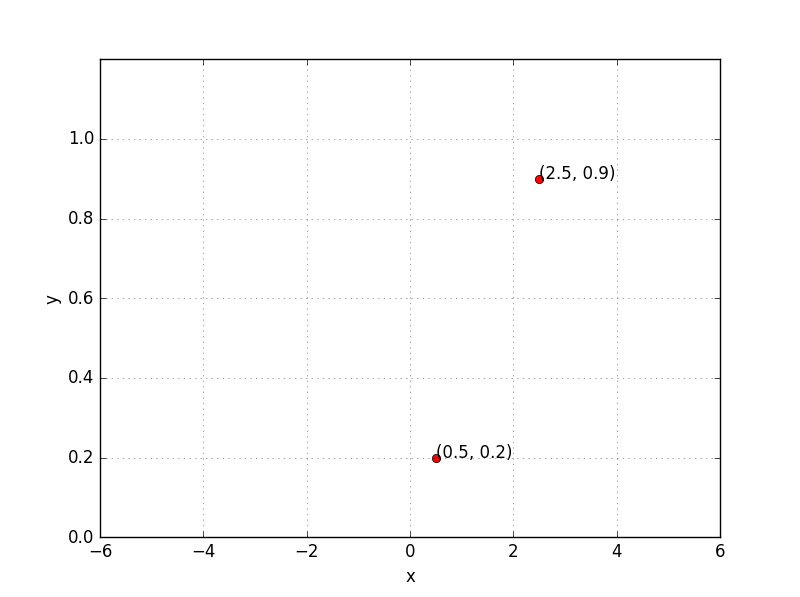
\includegraphics[scale=0.3]{images/module4/2sample_points.png}
				\end{center}
			\end{figure}
		\end{overlayarea}

		\column{0.5\textwidth}<2->
		\begin{overlayarea}{\textwidth}{\textheight}
			\begin{align*}
				\onslide<2->{\intertext{Let's assume there is only 1 point to fit $(x, y)$}}
				\onslide<3->{\mathscr{L}(w,b)                                       & = \frac{1}{2} * (f(x) - y)^2 \\}
				\onslide<4->{\nabla w = \frac{\partial\mathscr{L}(w,b)}{\partial w} & = \frac{\partial}{\partial w} [\frac{1}{2} * (f(x) - y)^2] \\}
			\end{align*}
		\end{overlayarea}
	\end{columns}
\end{frame}

\begin{frame}
	\begin{columns}
		\begin{column}{0.46\textwidth}
			\begin{overlayarea}{\textwidth}{\textheight}
				\begin{align*}
					\onslide<1->\nabla w & = \frac{\partial}{\partial w} [\frac{1}{2} * (f(x) - y)^2]                                                \\
					\onslide<2->{        & = \frac{1}{2} * [2*(f(x) - y) * \frac{\partial}{\partial w}(f(x) - y)] \\}
					\onslide<3->{        & = (f(x) - y) * \frac{\partial}{\partial w}(f(x)) \\}
					\onslide<4->{        & = (f(x) - y) * \frac{\partial}{\partial w}\Big(\frac{1}{1 + e^{-(wx + b)}}\Big) \\}
					\onslide<10->{       & = \color{red}{(f(x) - y) * f(x)*(1- f(x)) *x}}
				\end{align*}
			\end{overlayarea}
		\end{column}
		\vrule{}
		\begin{column}{0.54\textwidth}
			\begin{overlayarea}{\textwidth}{\textheight}
				\begin{align*}
					\onslide<5->{ & \frac{\partial}{\partial w}\Big(\frac{1}{1 + e^{-(wx + b)}}\Big) \\}
					\onslide<6->{ & =\frac{-1}{(1 + e^{-(wx + b)})^2}\frac{\partial}{\partial w}(e^{-(wx + b)})) \\}
					\onslide<7->{ & =\frac{-1}{(1 + e^{-(wx + b)})^2}*(e^{-(wx + b)})\frac{\partial}{\partial w}(-(wx + b))) \\}
					\onslide<8->{ & =\frac{-1}{(1 + e^{-(wx + b)})}*\frac{e^{-(wx + b)}}{(1 + e^{-(wx + b)})} *(-x) \\}
					\onslide<9->{ & =\frac{1}{(1 + e^{-(wx + b)})}*\frac{e^{-(wx + b)}}{(1 + e^{-(wx + b)})} *(x) \\}
					\onslide<10->{ & =f(x)*(1- f(x))*x}
				\end{align*}
			\end{overlayarea}
		\end{column}
	\end{columns}
\end{frame}

\begin{frame}
	\begin{columns}
		\column{0.45\textwidth}
		\begin{overlayarea}{\textwidth}{\textheight}
			\begin{tikzpicture}
	\node [neuron] (neuron0) at (1,6)  {$\sigma$} ;
	\node (input1) at (-1,6)  {$x$};
	\node (input0) at (-1,5)  {$1$};
	\node (output0) at (3,6)  {$y = f(x)$};
	\node (formula) at (0,4) {$f(x)= \frac{1}{1+e^{-(w\cdot x + b)}}$};
	\draw [->] (input0) -- (neuron0);
	\draw [->] (input1) -- (neuron0);
	\draw [->] (neuron0) -- (output0);
\end{tikzpicture}
			\vspace{-0.2in}
			\begin{figure}[!htp]
				\begin{center}
					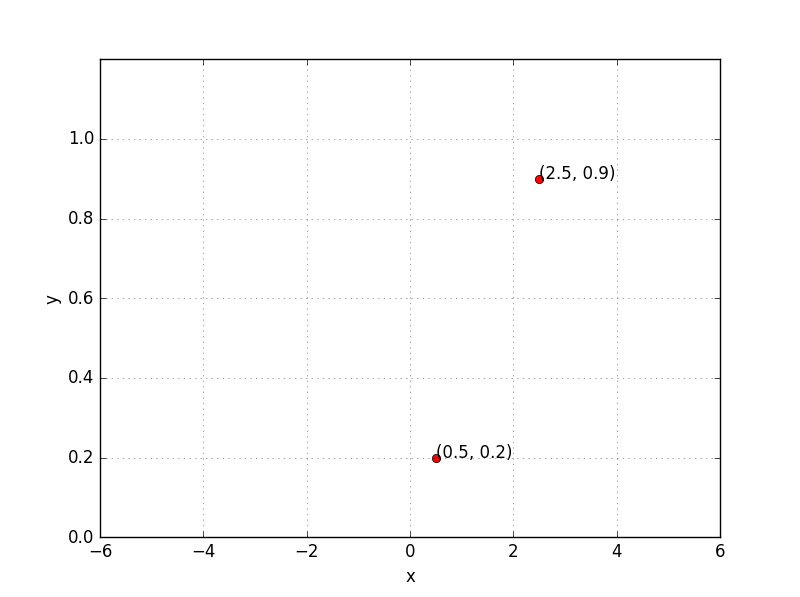
\includegraphics[scale=0.3]{images/module4/2sample_points.png}
				\end{center}
			\end{figure}
		\end{overlayarea}
		\column{0.55\textwidth}
		\begin{overlayarea}{\textwidth}{\textheight}
			\begin{align*}
				\onslide<1->{\intertext{So if there is only 1 point $(x, y)$, we have, }}
				\onslide<2->{\nabla w & = (f(x) - y) * f(x)*(1- f(x)) *x}
				\onslide<3->{\intertext{For two points,}}
				\onslide<4->{\nabla w & = \sum_{i=1}^{2} (f(x_i) - y_i) * f(x_i)*(1- f(x_i)) *x_i} \\
				\onslide<5->{\nabla b & = \sum_{i=1}^{2} (f(x_i) - y_i) * f(x_i)*(1- f(x_i))}
			\end{align*}
		\end{overlayarea}
	\end{columns}
\end{frame}


\begin{frame}
	\begin{columns}
		\column{0.5\textwidth}
		\begin{overlayarea}{\textwidth}{\textheight}
			\vspace{-0.15in}
			\begin{figure}
				\includegraphics<1>[clip,trim=0 650 0 0,scale=0.3]{images/module4/pseudo_code_sgd_crop.png}
				\includegraphics<2>[clip,trim=0 580 0 0,scale=0.3]{images/module4/pseudo_code_sgd_crop.png}
				\includegraphics<3-4>[clip,trim=0 415 0 0,scale=0.3]{images/module4/pseudo_code_sgd_crop.png}
				\includegraphics<5>[clip,trim=0 325 0 0,scale=0.3]{images/module4/pseudo_code_sgd_crop.png}
				\includegraphics<6>[clip,trim=0 235 0 0,scale=0.3]{images/module4/pseudo_code_sgd_crop.png}
				\includegraphics<7>[scale=0.3]{images/module4/pseudo_code_sgd_crop.png}
			\end{figure}
		\end{overlayarea}
		\column{0.5\textwidth}
		\begin{overlayarea}{\textwidth}{\textheight}
			\begin{figure}
				\includegraphics<4->[scale=0.5]{images/module4/error_surface1.png}
			\end{figure}
		\end{overlayarea}
	\end{columns}
\end{frame}


\begin{frame}
	\begin{columns}
		\column{0.5\textwidth}
		\begin{overlayarea}{\textwidth}{\textheight}
			\vspace{-0.15in}
			\begin{figure}
				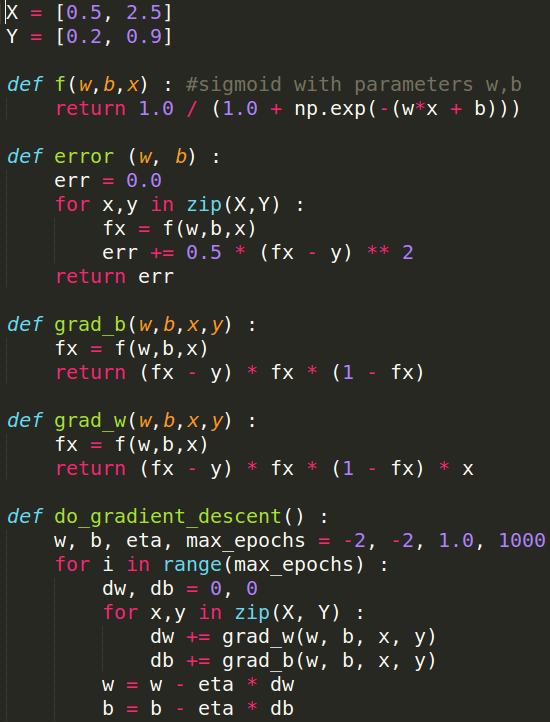
\includegraphics[scale=0.3]{images/module4/pseudo_code_sgd_crop.png}
			\end{figure}
		\end{overlayarea}
		\column{0.5\textwidth}
		\begin{overlayarea}{\textwidth}{\textheight}
			\vspace{-0.15in}
			\begin{figure}
				\foreach \n in {0,...,99} {%
						\includegraphics<\n>[scale=0.5]{images/module4/sgd0/sgd_error\n.png}
					}
			\end{figure}
		\end{overlayarea}
	\end{columns}
\end{frame}

\begin{frame}
	\begin{itemize}\justifying
		\item<1-> Later on in the course we will look at gradient descent in much more detail and discuss its variants
		\item<2-> For the time being it suffices to know that we have an algorithm for learning the parameters of a sigmoid neuron
		\item<3-> So where do we head from here ?
	\end{itemize}
\end{frame}